\documentclass[11pt,center]{beamer}

\usepackage{fancybox}
\usepackage{graphics}
\usepackage{spot}
\usepackage{tikz}
\usepackage{minibox}
\usetikzlibrary{arrows}
\usepackage[absolute,overlay]{textpos}
\usetheme{metropolis}

\usepackage[export]{adjustbox}

\definecolor{light-gray}{gray}{0.86}
\title{\huge{Adaptive Machine Learning}}
\author{Βασίλειος Αταλόγλου \\ Κωνσταντίνος Σαμαράς-Τσακίρης}
\date{\today}

\begin{document}

  \begin{frame}%{\maketitle}
	  \titlepage
  \end{frame}

\section{Προσομοιώσεις - Αποτελέσματα}

	\begin{frame}{Τεχνητά δεδομένα}
		Δημιουργία set ακολουθιών:
		\begin{itemize}
			\item[--]Απλή πρόβλεψη (A)
			\item[--]Πολλαπλή πρόβλεψη (B)
		\end{itemize}
		\vfill
		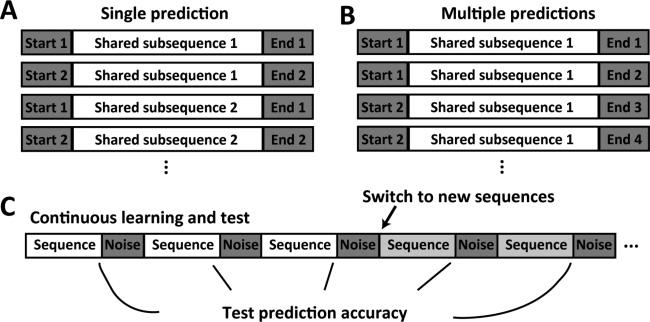
\includegraphics[width=0.6 \textwidth,center]{../pics/sequences.jpg}
		\vfill
		\pause
		Προσθήκη θορύβου ανάμεσα στις ακολουθίες
	\end{frame}
	
	
	
	\begin{frame}{Τεχνητά δεδομένα}
		Σύγκριση διαφορετικών υλοποιήσεων για μονή πρόβλεψη:\\
		\vspace{1em}
		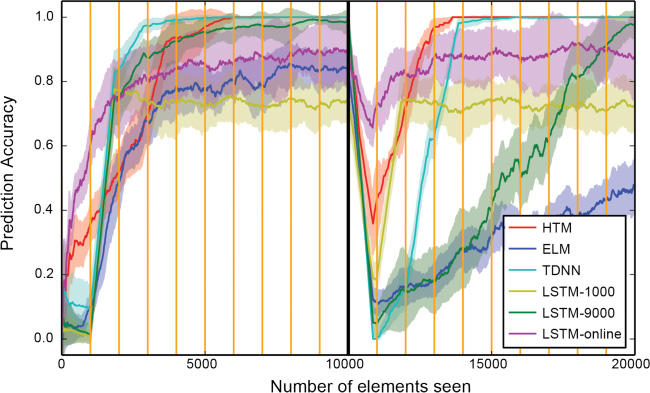
\includegraphics[width=0.7 \textwidth,center]{../pics/single_prediction.jpg}
		\pause
		\begin{tabbing}
  			Το HTM:  \=α) πετυχαίνει perfect accuracy\\
  			\>β) προσαρμόζεται στις αλλαγές του περιβάλλοντος\\
  		\end{tabbing}
	\end{frame}
	
	\begin{frame}{Τεχνητά δεδομένα}
		Πολλαπλές προβλέψεις:
		\vfill
		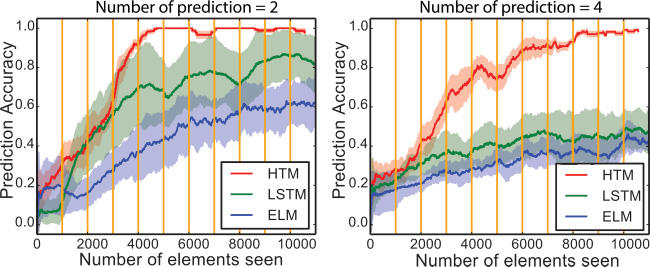
\includegraphics[width=0.7 \textwidth,center]{../pics/multiple_predictions.jpg}
		\pause
		\vfill
		To HTM είναι το \alert{μόνο} που πετυχαίνει perfect accuracy.\\
		\pause
		Αιτία: Αναπαράσταση με \textbf{SDR} !!
	\end{frame}
	
	\begin{frame}{Τεχνητά δεδομένα}
		\begin{columns}
		\column {0.4 \textwidth}
		\\
			\visible<1->{
			Πρόβλεψη high-order ακολουθιών} \\
			\vspace{5em}
			\visible<2->{
			Ανθεκτικότητα σε κατεστραμμένο δίκτυο}
		\column {0.6 \textwidth}
			\vspace{1em}
			\visible<1->{
			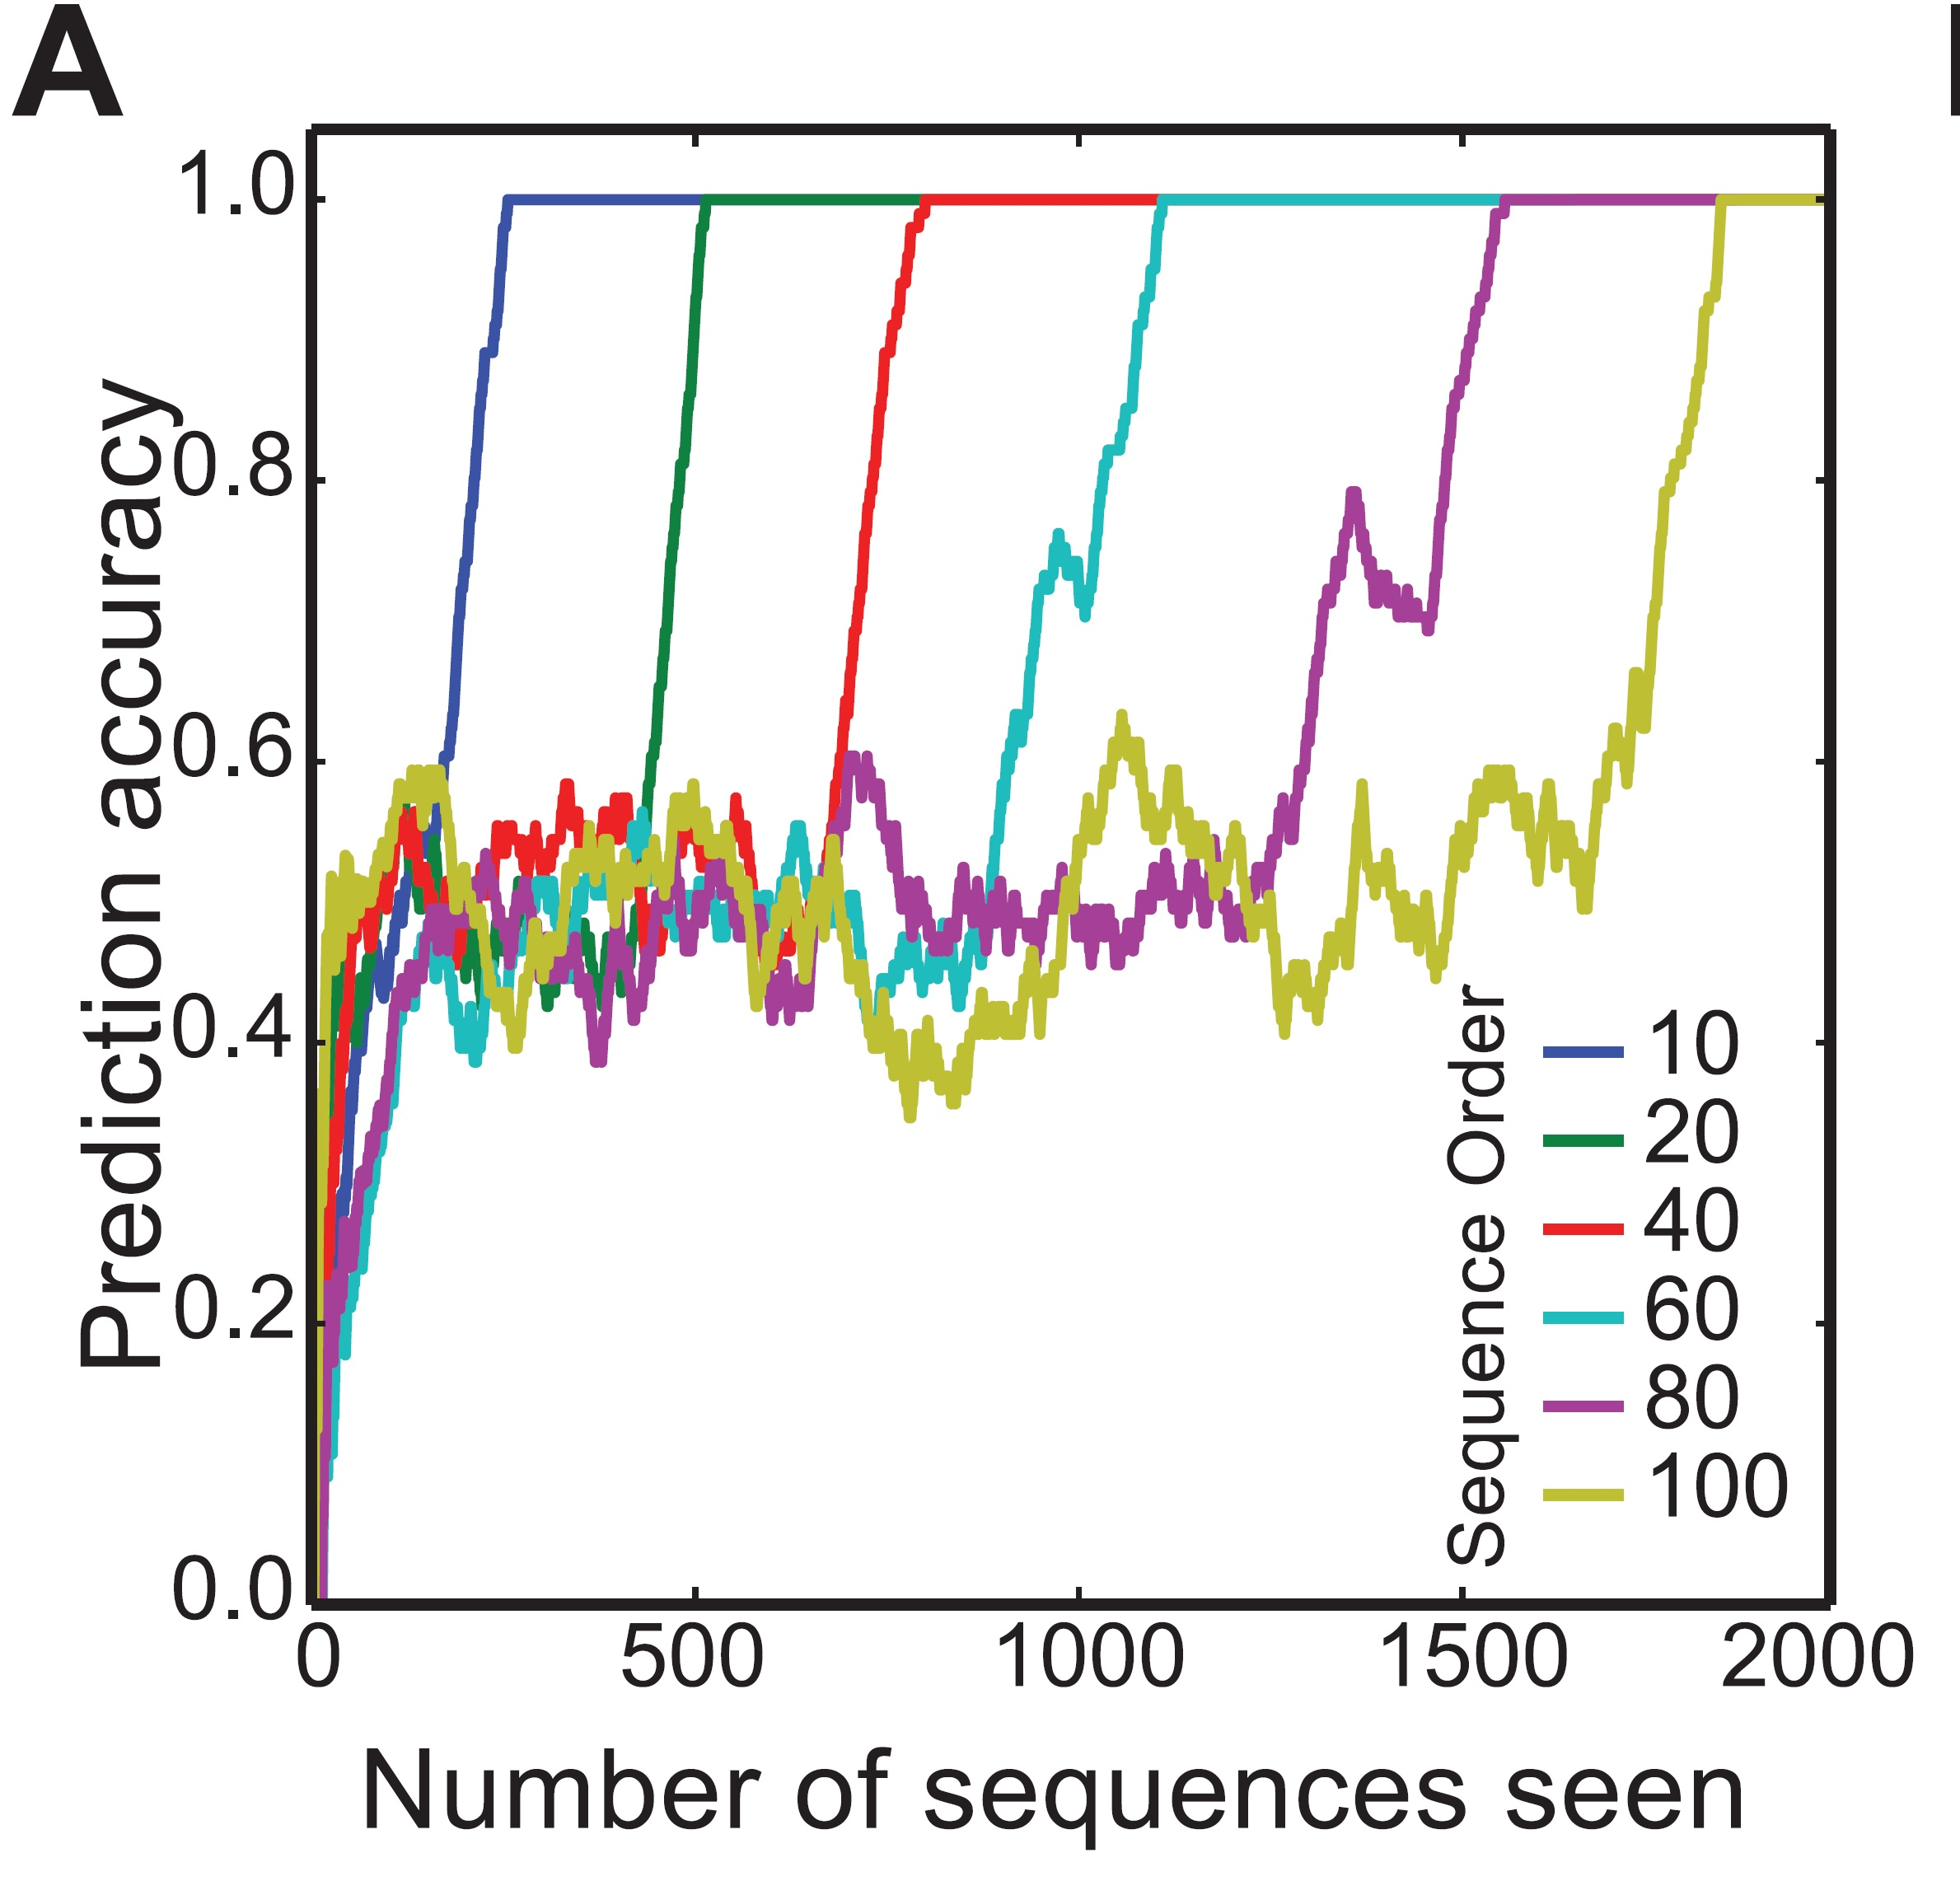
\includegraphics[width=0.6 \textwidth,center]{../pics/sequence_order.jpg}}
			\vspace{0.5em}
			\visible<2->{
			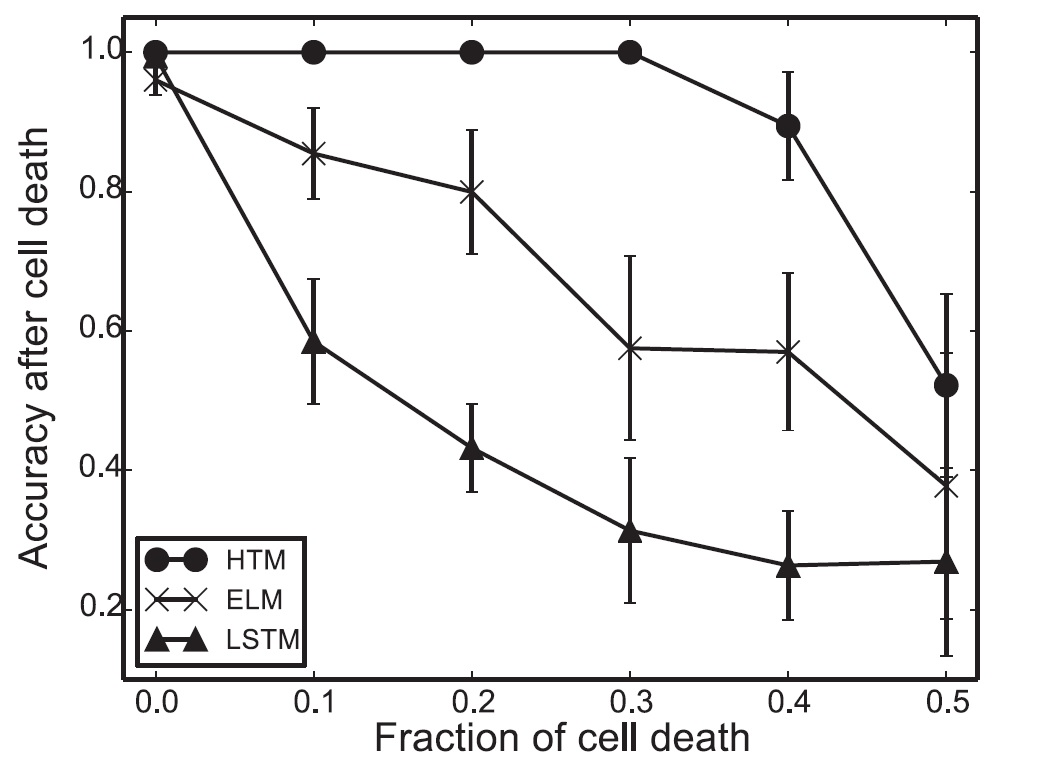
\includegraphics[width=0.65 \textwidth,center]{../pics/cell_death.jpg}}
		\end{columns}
	\end{frame}
	
	\begin{frame}{Πραγματικά δεδομένα}
		Ζήτηση ταξί Νέας Υόρκης (διάστημα 30 λεπτών)
		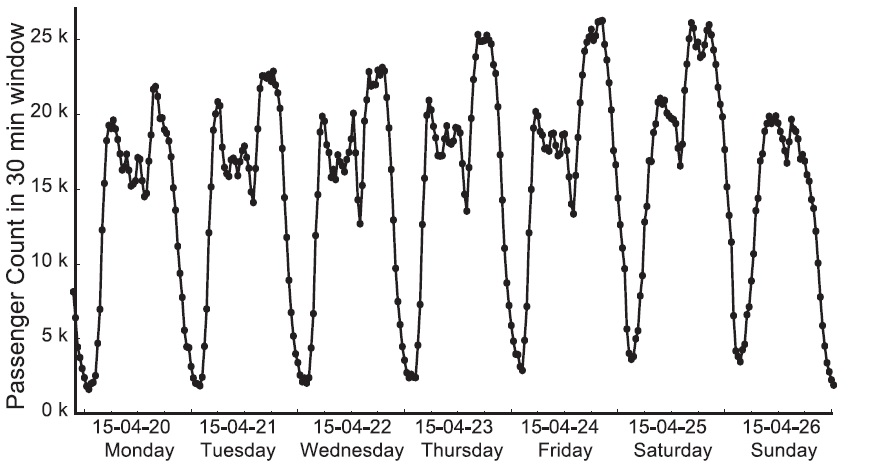
\includegraphics[width=0.5 \textwidth,center]{../pics/taxi_demand.jpg}
		\vfill
		\pause
		\begin{columns}
		\column {0.5 \textwidth}
			Στόχος: Πρόβλεψη της ζήτησης 2.5 ώρες πριν
		\column {0.4 \textwidth}
			\vspace{1em}
			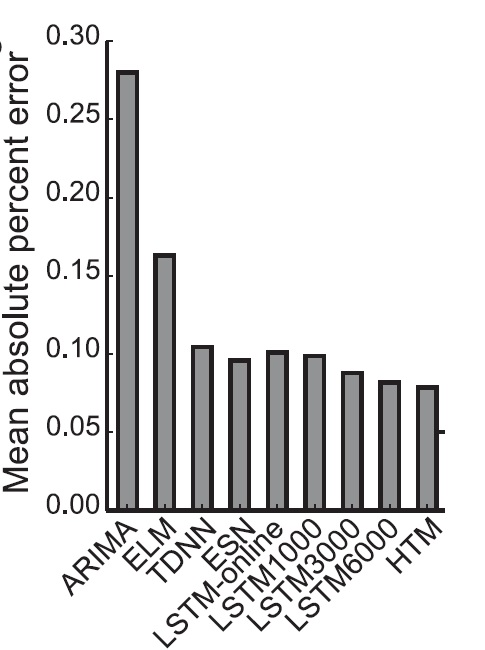
\includegraphics[width=0.6 \textwidth,left]{../pics/taxi_accuracy.jpg}
		\end{columns}
	\end{frame}
	
	
	
\section{Hardware}
	
	
	\begin{frame}{SpiNNaker Chip}
		Yψηλής παραλληλοποίησης υπολογιστικό σύστημα για την μοντελοποίηση και προσομοίωση spiking 				neural networks.
		\pause
		\vfill
		Βασικό στοιχείο το SpiNNaker Chip Multiprocessor (CMP):
		\vfill
		\begin{columns}
			\column{0.5 \textwidth}
			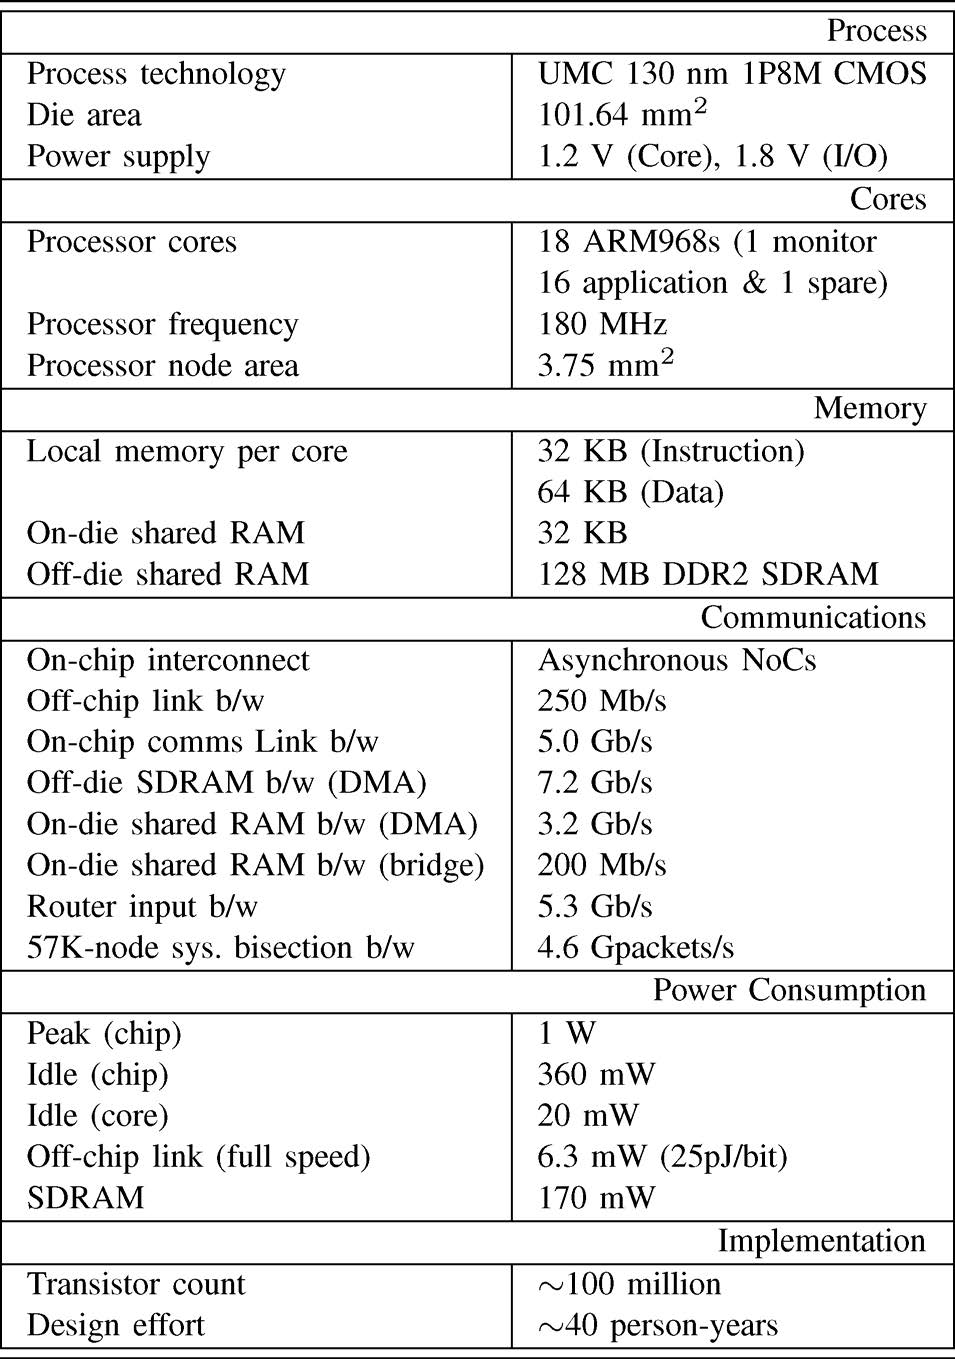
\includegraphics[width=0.75 \textwidth,right]{../pics/CMPspecs.jpg}
			\column{0.5 \textwidth}
			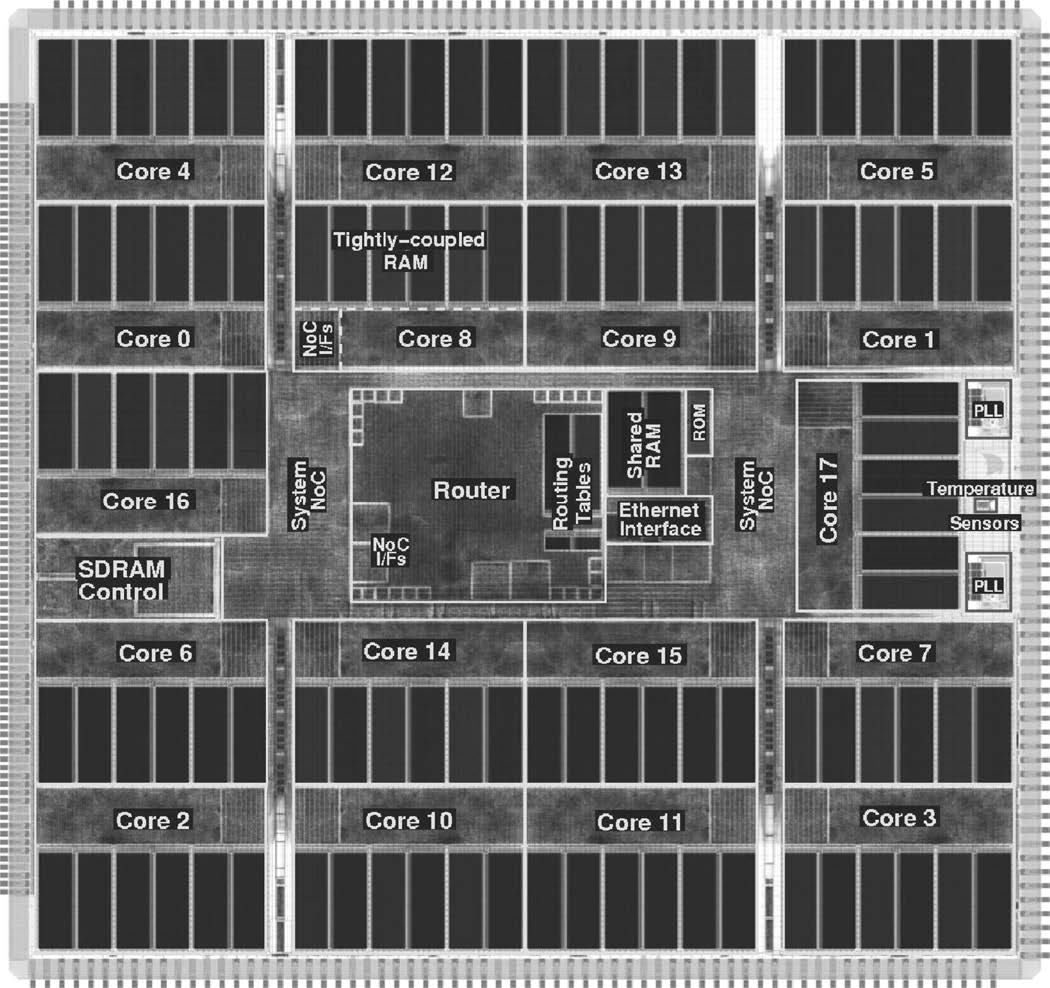
\includegraphics[width=0.75 \textwidth,left]{../pics/CMP.jpg}
		\end{columns}
	\end{frame}
	
	\begin{frame}{SpiNNaker Network}
		SpiNNaker: Πίνακας από κόμβους που περιέχουν CMP και 128MB SDRAM σε κοινό package.
		\pause
		\vfill
		Συνολικά, έχουμε:
		\begin{columns}
			\column{0.6 \textwidth}
				\begin{itemize}
					\item[--] 57600 CMPs
					\item[--] $10^6$ ARM968
					\item[--] $10^{9}$ νευρώνες ($1 \%$ εγκεφάλου)
					\item[--] 228 TIPS
					\item[--] 90KW ισχύς
				\end{itemize}
			\column{0.5 \textwidth}
				\includegraphics[width=0.9 \textwidth,left]{../pics/SpiNNaker.jpg}
		\end{columns}
	\end{frame}
	
	\begin{frame}{Χαρακτηριστικά SpiNNaker}
		\begin{description}[Sensor output]
			  \item[Επικοινωνία] Address Event Representation (AER), NoC
			  \pause
			  \vfill
			  \item[Μνήμη] Fast-access για την κατάσταση του νευρώνα\\
			  SDRAM για την κατάσταση των συνάψεων
			  \pause
			  \vfill
			  \item[Κατανάλωση] Ασύγχρονη Επικοινωνία\\
			  Sleep mode στην idle κατάσταση \\
			  Επιλογή ARM968 και SDRAM
		\end{description}
	\end{frame}
	
	\begin{frame}{Παράδειγμα υλοποίησης}
		Σύστημα για classification χειρόγραφων ψηφίων (MNIST database) μέσω Deep Neural Network
		\vspace{1em}
		\pause
		\begin{columns}
		\column {0.4 \textwidth}
			\begin{itemize}
			\item<2->[--] Ακρίβεια
			\item<3->[--] Ισχύς: 0.3 Watt
			\item<4->[--] Latency 
			\end{itemize}
			
		\column {0.6 \textwidth}
		\visible<2->{
		\\
			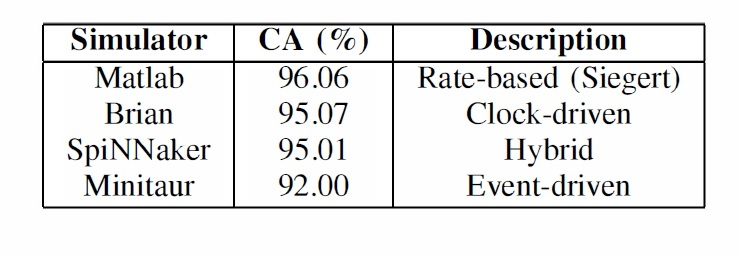
\includegraphics[width=0.8 \textwidth,left]{../pics/Accuracy.jpg}
		}
			\vspace{0em}
		\visible<4->{
			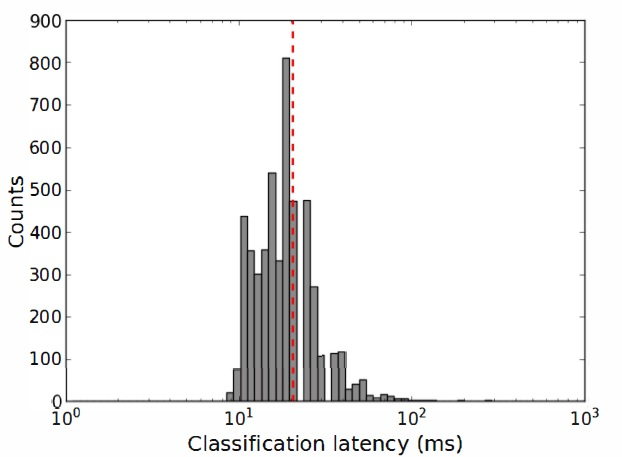
\includegraphics[width=0.8 \textwidth,left]{../pics/Latencies.jpg}
		}
		\end{columns}
		
		
		
	\end{frame}
	
	\begin{frame}{BrainScaleS Project (BSS)}
	Υβριδική πλατφόρμα: Cluster + Νευρομορφικό σύστημα
	\vfill
	\pause
	Βασικό στοιχείο: High Input Count Analog Neural Network (HICANN)
	\vfill
	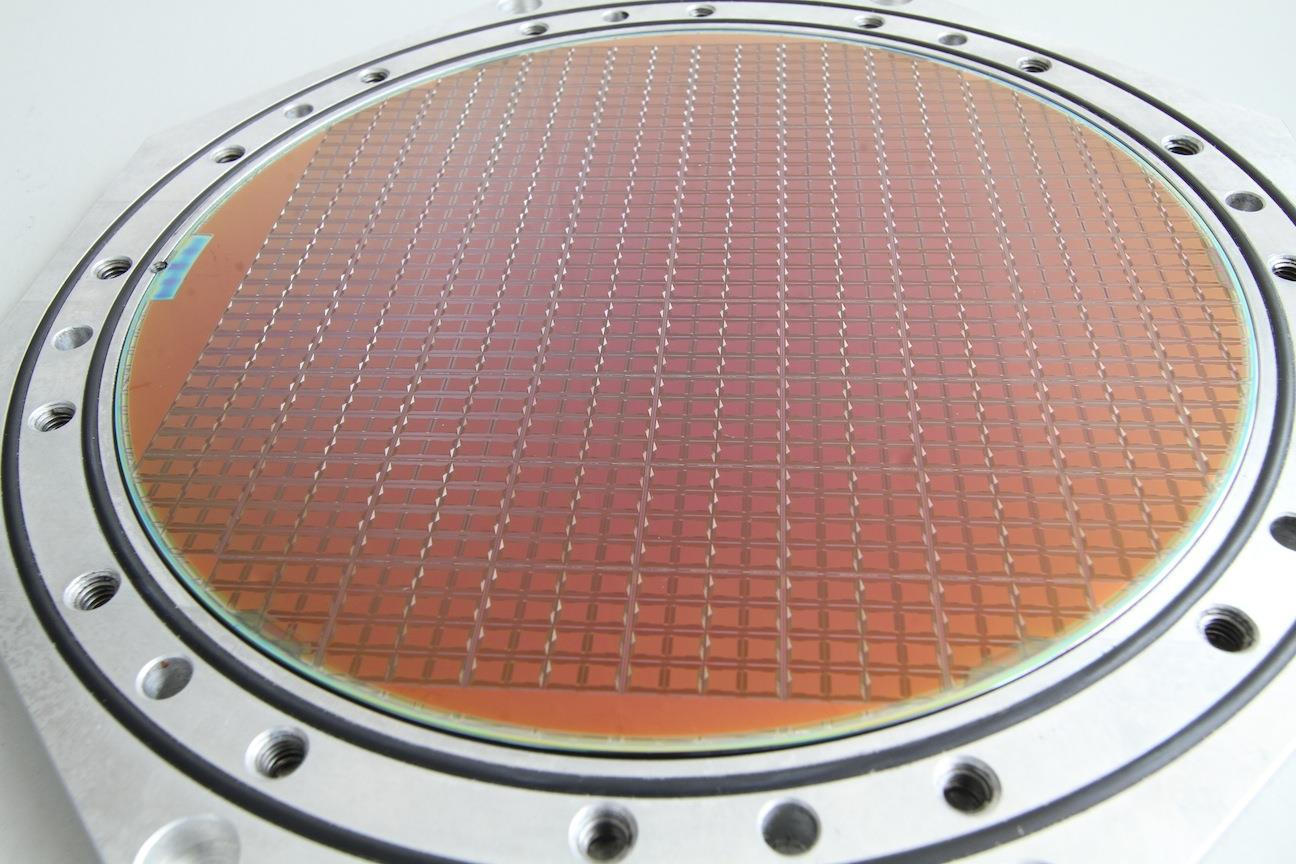
\includegraphics[width=0.4 \textwidth,center]{../pics/HICANN.jpg}
	\pause
	\vfill
	Mixed-signal: Αναλογικά νευρωνικά κυκλώματα, Ψηφιακή επικοινωνία
	\end{frame}
	
	\begin{frame} {HICANN chip}
		Κάθε HICANN chip:
		\begin{itemize}
			\item[--] 512 νευρώνες τύπου AdEx
			\item[--] 2 ομάδες 226 συνάψεων (πχ. proximal, distal)
		\end{itemize}
		\pause
		\vfill
		Ένα wafer περιέχει $364$ HICANN chips, δηλαδή:
		\begin{itemize}
			\item[--] $200\cdot 10^3$ νευρώνες
			\item[--]$45\cdot 10^6$ συνάψεις
		\end{itemize}
		\pause
		\vfill
		Η σημερινή πλατφόρμα αποτελείται 20 wafers.
		
	\end{frame}
	
	\begin{frame} {HICANN Chip}
		\begin{columns}
		\column {0.5 \textwidth}
			\begin{itemize}
				\item<1->[--]Motherboard πάνω\\ από το wafer
				\item<1->[--]FPGA για inter-wafer επικοινωνία
			\end{itemize}
			\vspace{5em}
			\begin{itemize}
				\item<2->[--]Διαχωρισμός σε reticles
				\item<2->[--]Συνδέσεις μέσω πυκνού δικτυώματος από wires
			\end{itemize}
			
		\column {0.5 \textwidth}
			\visible<1->{
			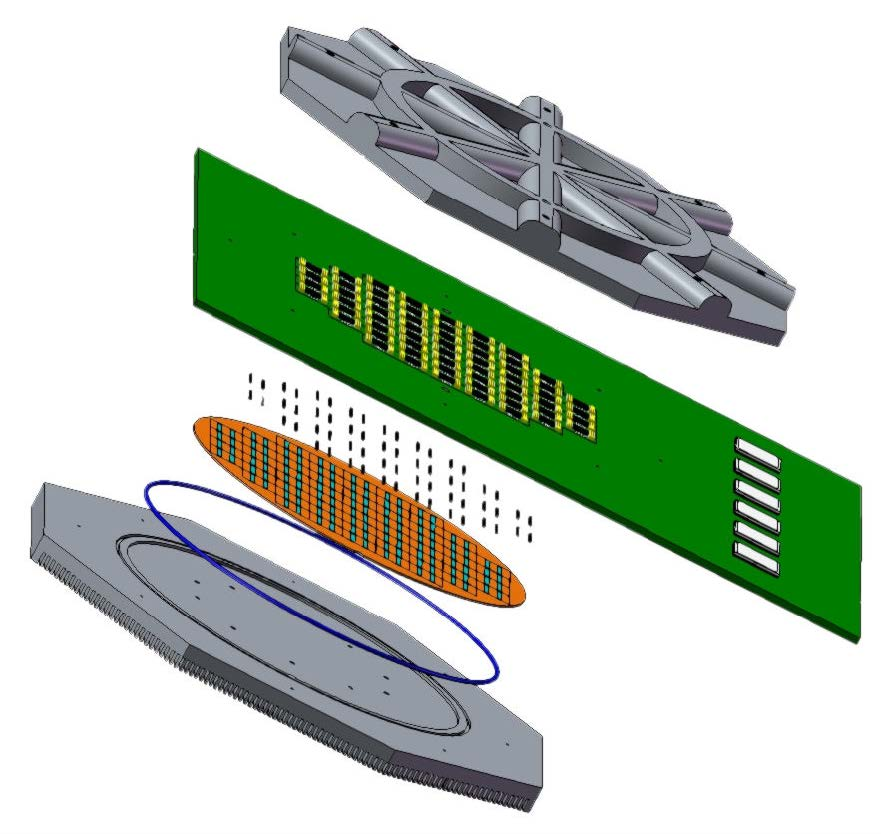
\includegraphics[width=0.7 \textwidth,left]{../pics/wafer.jpg}}
			\vspace{1em}
			\visible<2->{
			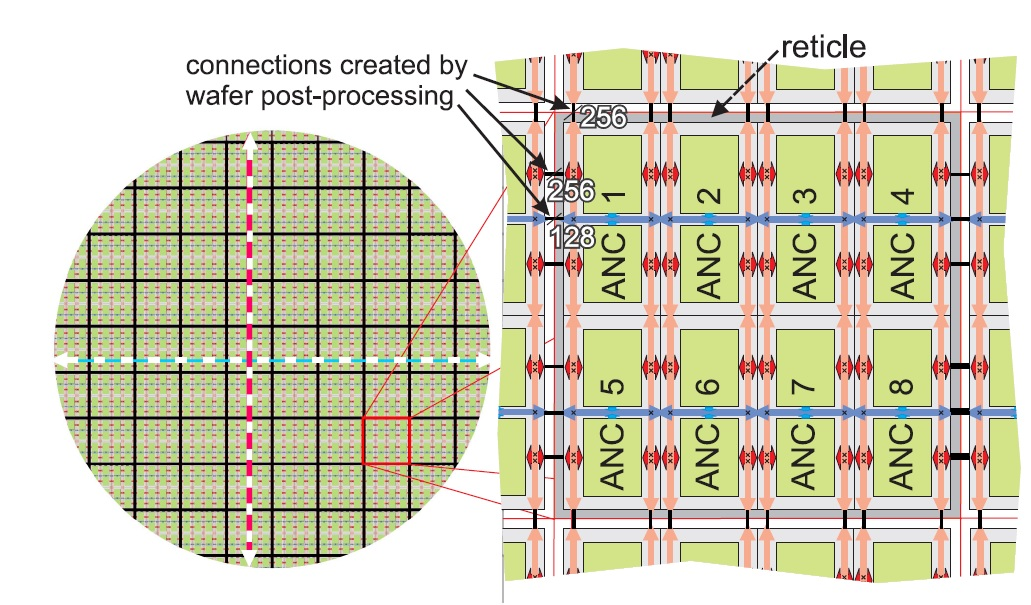
\includegraphics[width=0.8 \textwidth,left]{../pics/reticle.jpg}}
		\end{columns}
	\end{frame}
	
	\begin{frame} {HICANN Chip}
		\begin{columns}
		\column {0.5 \textwidth}
			\begin{itemize}
				\item<1->[--] Κυκλώματα μεμβράνης
				\item<2->[--] Είσοδος από synapse driver
				\item<3->[--] Strobe lines
				\item<4->[--] Neuron builder
			\end{itemize}
		\column {0.6 \textwidth}
			\visible<1->{
			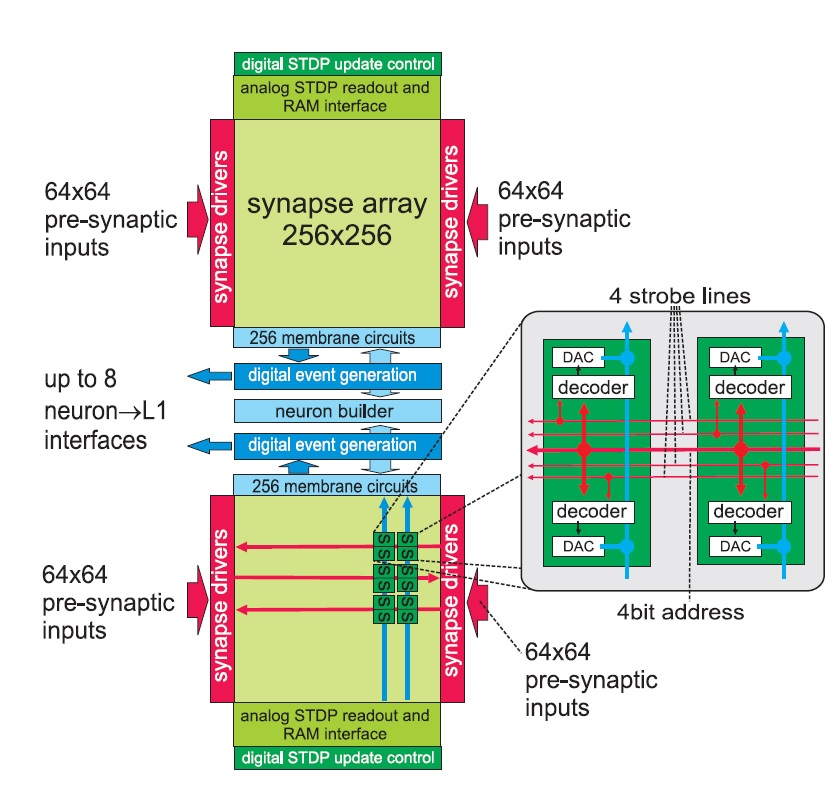
\includegraphics[width=0.9 \textwidth,left]{../pics/insideHICANN.jpg}}
			\end{columns}
	\end{frame}
	
	\begin{frame}{Συνάψεις}
			\begin{itemize}
				\item<1->[--]4 bit SRAM για το βάρος
				\item<1->[--]Ρεύμα ανάλογο του βάρους
				\item<1->[--]MUX για επιλογή εισόδου (excitatory/inhibitory)
			\end{itemize}
		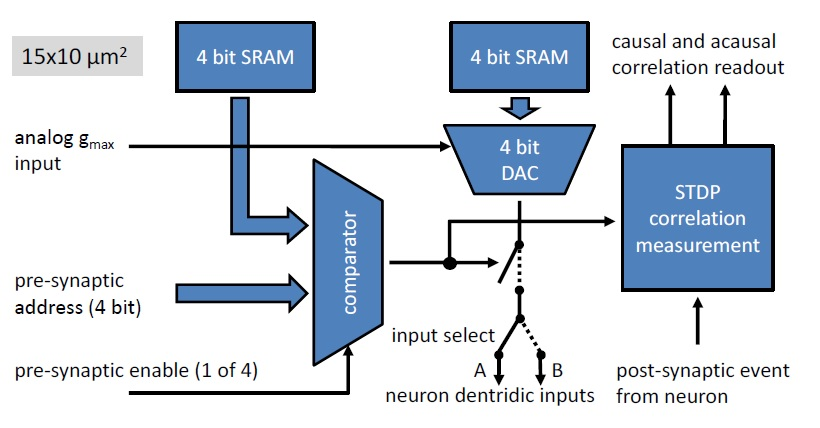
\includegraphics[width=0.8 \textwidth,center]{../pics/synapses.jpg}
	\end{frame}
	
	\begin{frame}{Adaptive Exponential Model}
		\begin{tabbing}
  			To AdEx περιγράφεται από 2 μεταβλητές:  \=α) Δυναμικό Μεμβράνης\\
  			\>β) Adaptation w
  		\end{tabbing}
  			\pause
  			Σε DC είσοδο παρουσιάζει την εξής συμπεριφορά:
  			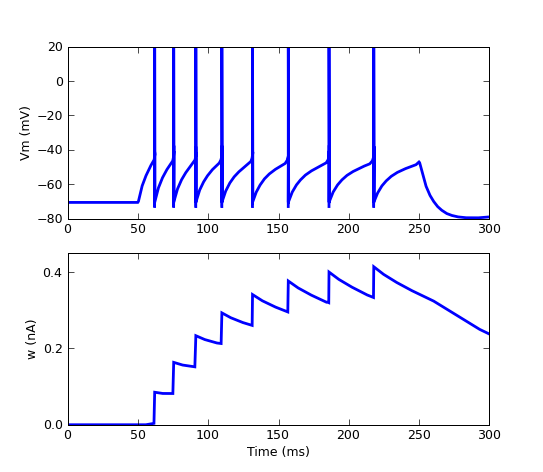
\includegraphics[width=0.4 \textwidth,center]{../pics/adex.jpg}
  			\pause
  			\vfill
  			Tο rise time εξαρτάται από το επίπεδο του input.

		 
	\end{frame}
	
	
	
	
	
	\begin{frame}{Υλοποίηση Spatial Pooler}
		Time - based σύστημα: Οι νευρώνες με το μεγαλύτερο input ενεργοποιούνται πρώτοι\\
		\vspace{2em}
		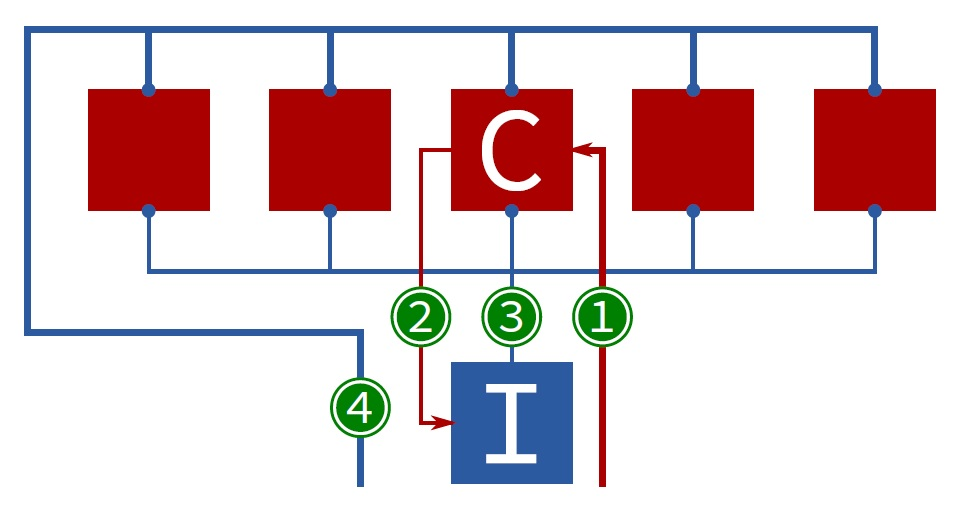
\includegraphics[width=0.5 \textwidth,center]{../pics/spatial_hardware.jpg}
		\pause
		\vfill
		\begin{tabbing}
  			Το inhibition cell(I):  \= α) διατηρεί τo sparsity\\
  			\> β) ελέγχει τη σταθερότητα\\
  		\end{tabbing}
	\end{frame}
	
	\begin{frame}{Υλοποίηση Temporal Pooler}
		\begin{columns}
		\column {0.6\textwidth}
			\begin{itemize}
				\item<1->[--] Ένα κελί (P) για το proximal input
				\item<1->[--] Μια τριάδα (D,I,S) για κάθε νευρώνα του multicolumn
				\vspace{1em}
				\item<2->[--] To Distal (D) αθροίζει τις συνάψεις "πρόβλεψης"
				\vspace{1em}
				\item<3->[--] Το Inhibition (I) καθορίζει ποιοι νευρώνες του ενεργού multicolumn 							ενεργοποιούνται
			\end{itemize}
			
		\column {0.4\textwidth}
			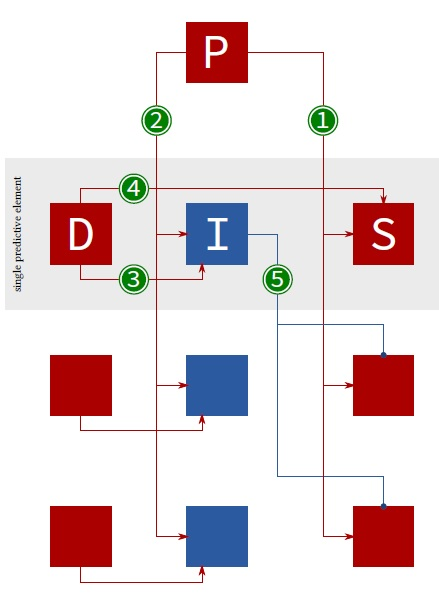
\includegraphics[width=1 \textwidth,center]{../pics/temporal_hardware.jpg}
		\end{columns}
		
	\end{frame}
	
	\begin{frame}{Αποτελέσματα προσομοιώσεων}
		\begin{columns}
		\column {0.5 \textwidth}
			\begin{itemize}
				\item<1->[--]Ενεργοποίηση νευρώνων με μεγαλύτερο overlap
			\end{itemize}
			\vspace{5em}
			\begin{itemize}
				\item<2->[--]Διατήρηση συσχετίσεων εισόδου-εξόδου
			\end{itemize}
			
		\column {0.5 \textwidth}
		
			\visible<1->{
			\vspace{1em}
			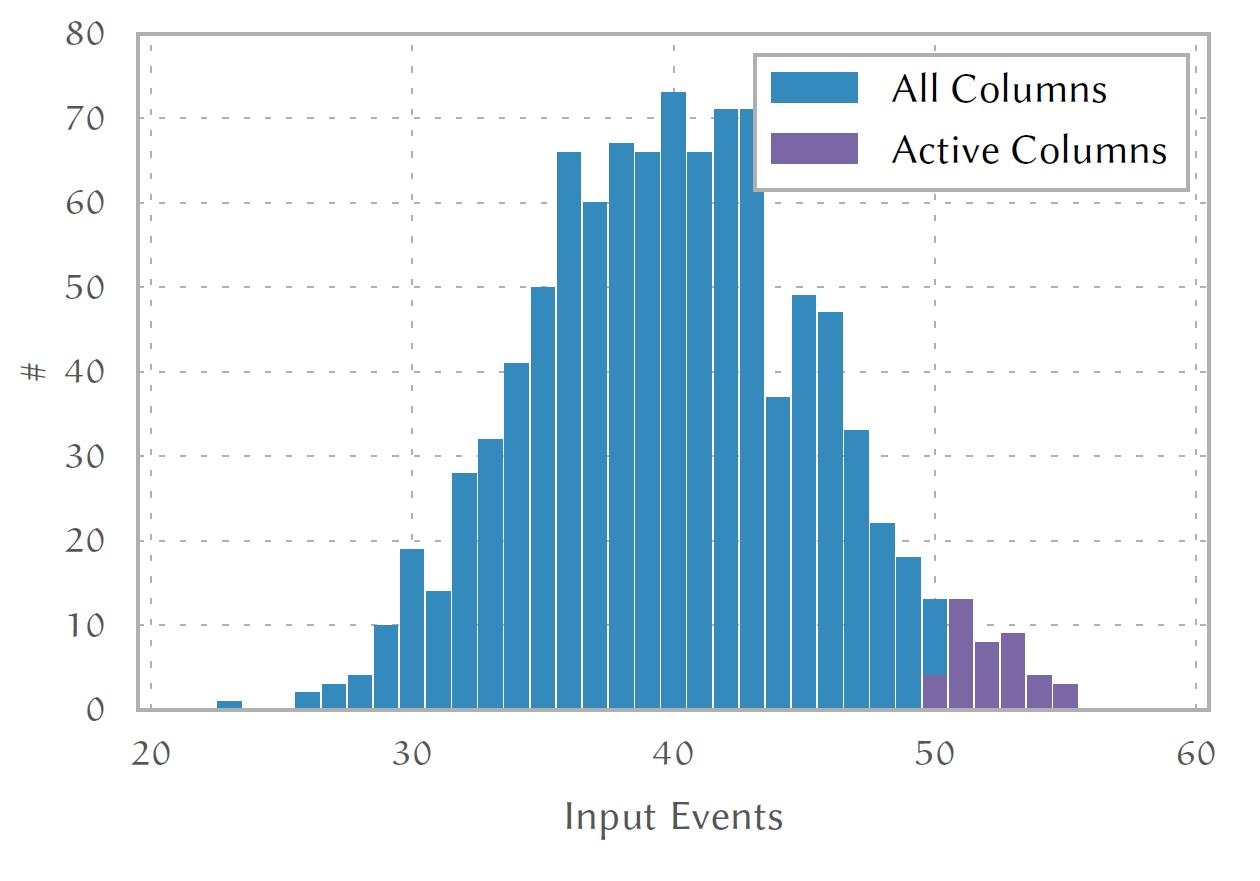
\includegraphics[width=0.9 \textwidth,left]{../pics/spatialsim1.jpg}}
			\vspace{0.5em}
			\visible<2->{
			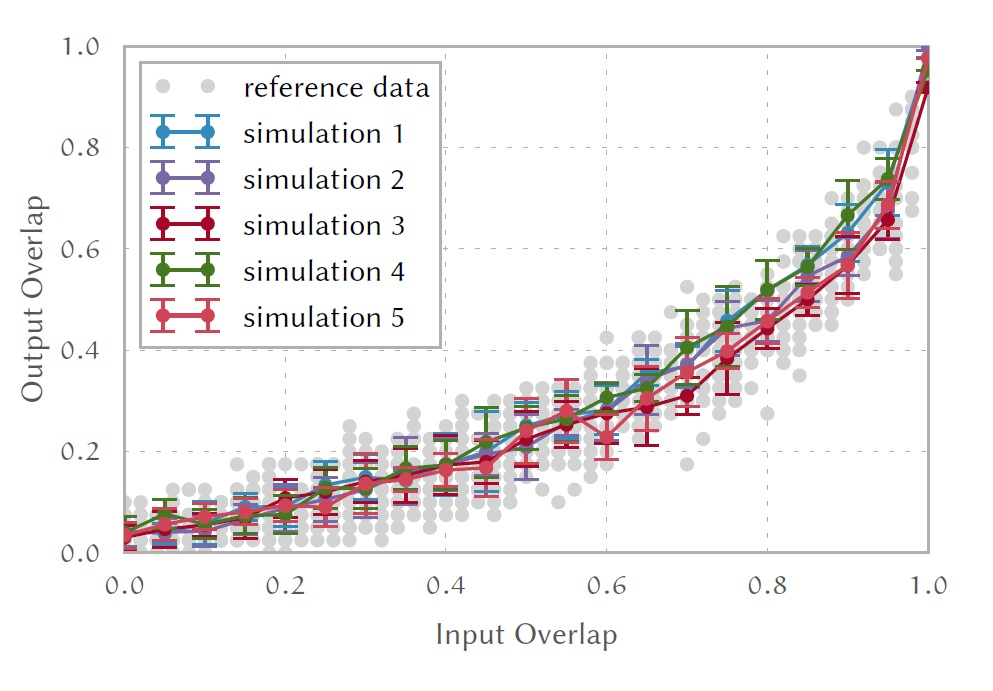
\includegraphics[width=0.9 \textwidth,left]{../pics/spatialsim2.jpg}}
		\end{columns}
	\end{frame}
	
	\begin{frame}{Βιβλιογραφία}
		\only<1>{
		[1] Y.LeCun, "Deep learning and convolutional networks", Hot Chips 27 Symposium (HCS), 2015 IEEE\newline
		[2] J.Hawkins and S.Ahmad, "Why Neurons Have Thousands of Synapses, a Theory of Sequence Memory in Neocortex",Front. Neural Circuits, 30 March 2016\newline
		[3] Y.Cui, S.Ahmad and J.Hawkins, "Continuous Online Sequence Learning with an Unsupervised
Neural Network Model", Neural Computation 28, 2474–2504 (2016)\newline
		[4] J. Schemmel, J. Fieres, and K. Meier, “Wafer-scale integration of analog neural networks,” in Proc. IEEE Int. Joint Conf. Neural Netw., Jun. 2008, pp. 431–438 \newline}
		\only<2>{
		[5]  E. Painkras, L. A. Plana, J. Garside, S. Temple, F. Galluppi, C. Patterson, D. R. Lester, A. D. Brown, and S. B. Furber, “Spinnaker: A 1-w 18-core system-on-chip for massively-parallel neural network simulation,” IEEE J. Solid-State Circuits, vol. 48, no. 8, pp. 1943–1953, Aug.2013\newline
		[6] Kanerva, P. (1988). Sparse Distributed Memory. Cambridge, MA: The MIT Press\newline
		[7] S.Billaudelle and S.Ahmad, Porting HTM Models to the Heidelberg Neuromorphic
Computing Platform \newline
		[8] HTM school: Video lectures provided on YouTube by Numenta}

		
	
	\end{frame}
	
	\begin{frame}
	\vspace{4em}
	\centering{\Huge{\textbf{ΕΥΧΑΡΙΣΤΟΥΜΕ ΓΙΑ ΤΗΝ ΠΡΟΣΟΧΗ ΣΑΣ}}}\\
	\vspace{3em}
	\centering{\normalsize{Αταλόγλου Βασίλειος\\
	Σαμαράς-Τσακίρης Κωνσταντίνος}}
	
	\end{frame}




\end{document}
